\section{Geschützplattform (Becker)}

Als Geschützplattform wird der Unterbau des Geschützes
bezeichnet, welcher den Geschützarm mit der Lochplatte des
Fahrzeugs verbindet. Diese Plattform besteht aus zwei,
3D-gedruckten Komponenten.

\subsection{Unterbau}

Der erste Teil des Objekts ist der Unterbau, welcher eine zylindrische Form aufweist und mit einer Bodenplatte versehen ist. 
Diese ist mit Schraublöchern ausgestattet, welche dazu dienen, den Aufbau mit dem Fahrzeug zu verbinden. 
Das vorliegende Bauteil wurde aus dem vorherigen Projekt übernommen, da die Konstruktion bereits auf dem Fahrzeug verbaut war 
und eine Eigenkonstruktion sehr ähnlich aufgebaut wäre.

Der Unterbau ist so konstruiert, dass er Platz für folgende Komponenten bietet:
\begin{itemize}
    \item Eine \textbf{PCA9685 PWM-Treiberplatine} zur Ansteuerung der
     Servomotoren auf dem Geschütz. Die erforderlichen Befestigungsbohrungen für die Platine waren bereits im Design integriert.
    \item Einen \textbf{MG996R Servomotor}, der für die Rotation des
     darüberliegenden Aufbaus verantwortlich ist.
\end{itemize}

\subsection{Abdeckung}
  
Die zweite Komponente ist die Abdeckung des Unterbaus. Diese
verfügt über Bohrungen zur Verbindung mit dem im Unterbau
positionierten Servomotor sowie über Montagepunkte für den
Geschützarm.

\begin{figure}[ht]
    \centering
    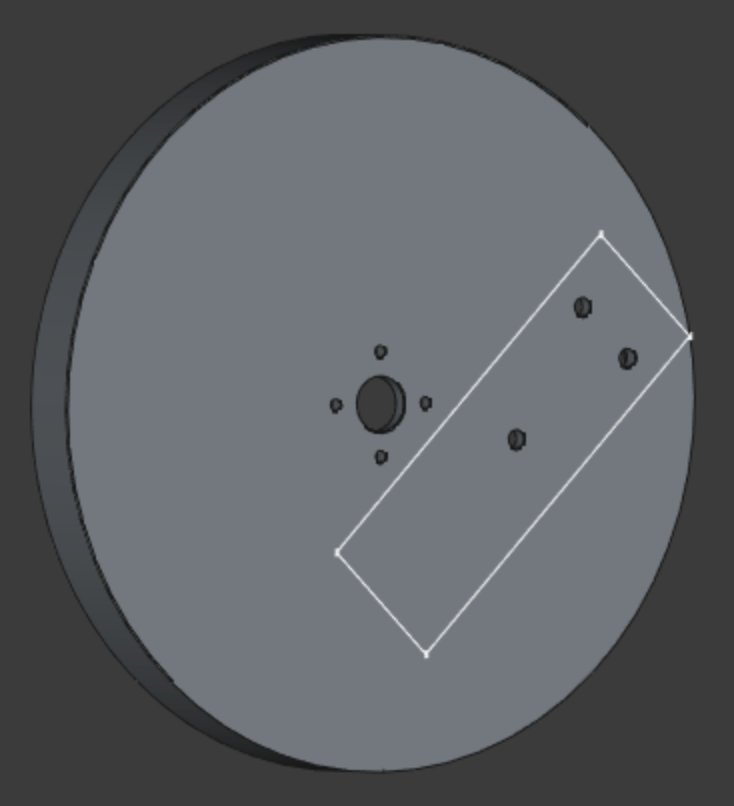
\includegraphics[width=0.35\textwidth, keepaspectratio]{images/becker_cad_platform.png}
    \caption{Abdeckung Plattform mit Position des Verbindungsstücks}
    \label{fig:cad_platform}
\end{figure}

Obwohl auch diese Abdeckung bereits vorhanden war, wurde sie
exakt vermessen und in FreeCAD rekonstruiert. Ziel dieser
Rekonstruktion war es, wie in Abbildung~\ref{fig:cad_platform} ersichtlich, die Bohrlöcher für die Verbindung mit dem
Geschützarm so zu positionieren, dass das Verbindungsstück und das
Magazin ohne weitere Anpassungen direkt montiert werden konnten.

\section{Magazin und Verbindungsstück (Becker)}

Das Magazin, sowie das Verbindungsstück wurden auf Basis einer bestehenden Konstruktionsvorlage \cite{cad_turret_blueprint} 3D-gedruckt. 
Das Verbindungsstück ist so ausgelegt, dass es einen weiteren MG996R Servomotor aufnimmt, welcher die vertikale Neigung des Geschützes
steuert.

Die Struktur des Magazins umfasste einen linken und einen rechten Teil, die in der Vorlage zusammengeklebt wurden.
Wie bereits im Abschnitt \ref{sec:cad_gunarm_v1} dargelegt, erfolgte für die Verbindung mit dem Geschützarm der ersten Version die Konstruktion von Verbindungsstücken an beiden Enden des Magazins, 
um mittels Schrauben eine Verbindung zwischen beiden Teilen zu gewährleisten.  Darüber hinaus wurden Schraublöcher in beide Teile des Magazins integriert, 
um eine Verbindung beider Teile mittels Schrauben zu ermöglichen.

In der zweiten Version des Geschützarmes wurden die Verbindungsstücke entfernt, da der Geschützarm nun direkt mit dem Magazin verbunden wird.
Die vorgenommene Änderung resultierte aus der Tatsache, dass es aufgrund der signifikant geringeren Dimension des Geschützarmes unmöglich war, Verbindungsstücke mit Schraublöchern zu versehen.

Zuletzt wurde auch die Länge des Laufs vergrößert, um eine bessere Stützung des Geschützarms zu gewährleisten.

\section{Magazingewicht (Becker)}

Das Magazin des Geschützes verfügt über eine Kapazität für sechs Nerf-Darts sowie ein Magazingewicht. 
Letzteres dient dazu, einerseits bei hoher Vibration des Fahrzeugs das Ausfallen der Darts zu verhindern und andererseits sicherzustellen, dass nach einem Schuss das nächste Geschoss nachrutscht.

Zunächst wurde die Vorlage \cite{cad_turret_blueprint} für das Magazingewicht angepasst, indem der Projektname eingraviert wurde.

\begin{figure}[ht]
    \centering
    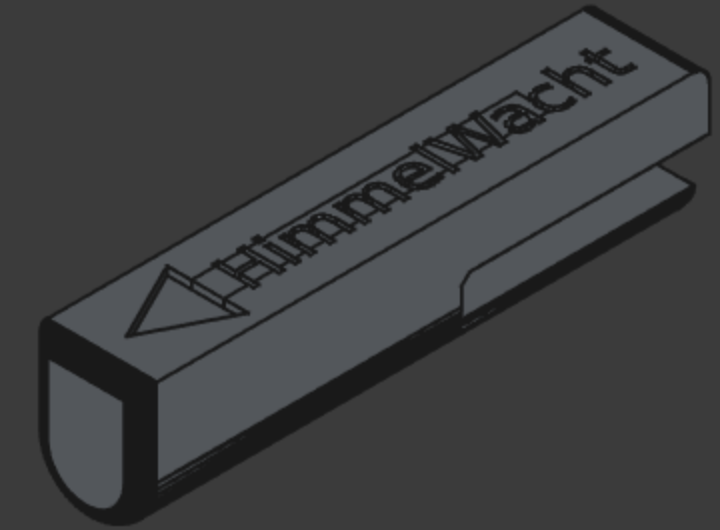
\includegraphics[width=0.35\textwidth, keepaspectratio]{images/cad_becker_weight.png}
    \caption{Magazingewicht}
\end{figure}

Das Gewicht besitzt außerdem eine Aussparung, die dafür sorgt, dass das Bauteil die Bewegung des Servo Motors nicht einschränkt, welcher die Darts bei der Schussabgabe in die Flywheel Motoren befördert. 
Ohne entsprechende Aussparung würde der Servo versuchen, das Gewicht in den Lauf zu schieben, was zu Materialschäden, entweder am Motor oder am Geschütz führen würde.

Die vorliegende Aussparung führte allerdings zu Problemen. Wird die Platform sehr weit nach hinten geneigt, so kam es vor, dass der hintere Teil des Gewichts nicht schwer genug war, um die Nerfs-Darts in den Lauf zu drücken.
Die Lösung für dieses Problem bestand im Einsatz selektiver Infill-Technik. Die übrigen Teile wurden standardmäßig mit einem Infill-Gehalt von 15\% gedruckt.
Im hinteren Teil des Gewichts wurde jedoch eine 100\% Infill eingesetzt. Dieses Vorgehen resultierte in der Behebung des Problems.

\section{Geschütztrigger (Becker)}

Der Auslösemechanismus initiiert den Schussvorgang. Durch die Aktivierung eines MG92B Servomotors wird ein Dart in die laufenden Flywheel-Motoren geschoben, welche ihn
beschleunigen und abfeuern.

Der Mechanismus ist eine zweiteilige Konstruktion, die auf einer bestehenden Vorlage \cite{cad_turret_blueprint} basiert, deren Schraublöcher jedoch für
den spezifischen Anwendungsfall angepasst wurden.

Am unteren Teil wurde eine Öffnung für eine M4-Schraube konstruiert, welche in das Magazin hineinreicht und Kraft auf den Dart ausübt. 
Bei der Verbindung der beiden Teile wurde darauf geachtet, dass das Schraubloch des ersten Teils etwas größer ist, so dass die Schraube hier nicht greift. 
Diese wird lediglich im zweiten Teil festgeschraubt, wodurch eine Art Gelenk entsteht.
Abschließend erfolgt noch die Verbindung des ersten Teils mit dem Servomotor.

\section{Halterungen Stormversorgung (Becker)}

Da einige Komponenten der Stromversorgung ebenfalls in ein früheres Projekt integriert wurden, wurde auch untersucht, wie die Vorgängergruppe diese Teile montiert hat.
Zu diesem Zweck hat die Gruppe Komponenten mit Stelzen gefertigt, die in die Lochplattform des Fahrzeugs eingesetzt werden konnten.

Dieses System wurde unter anderem für die Stromverteiler verwendet. 
Für dieses Projekt wurde ein weiteres Teil nach gleichem Prinzip für die Step-Down-Module erstellt, um auch diese in gleicher Weise befestigen zu können.

\begin{figure}[ht]
    \centering
    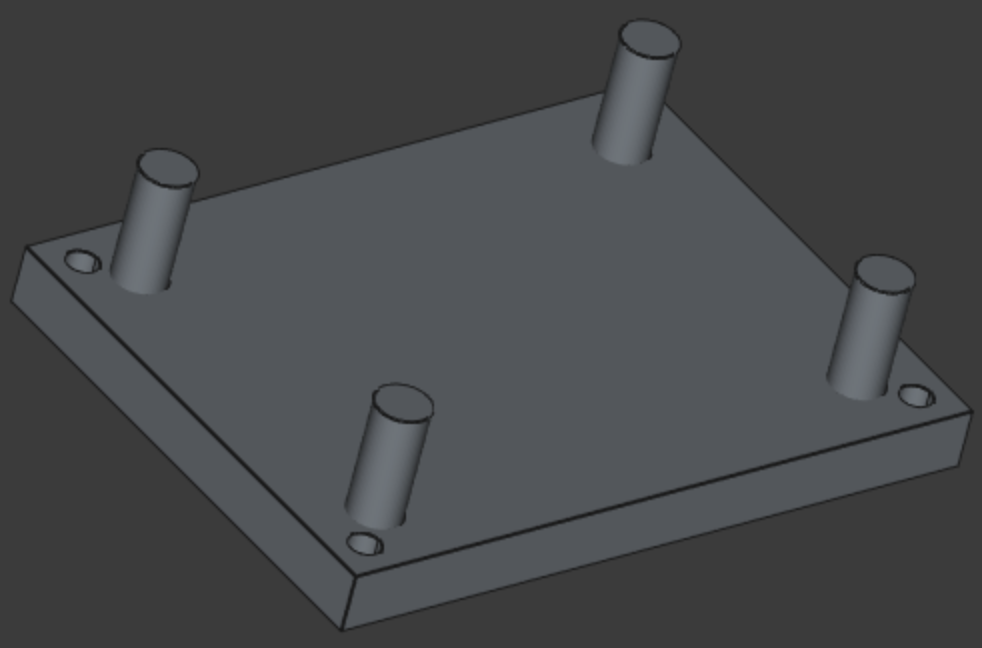
\includegraphics[width=0.35\textwidth, keepaspectratio]{images/becker_cad_powerplate.png}
    \caption{Halterung DC Step-Down mit Stecksystem}
\end{figure}

\section{Halterungen Flywheel Motortreiber (Becker)}

Des Weiteren wurde die Halterung für die Motortreiber der Flywheel-Motoren mit den gleichen Stempen ausgestattet. 
Die Halterung stellt eine modifizierte Version einer Vorlage \cite{cad_flywheel_blueprint} dar. 
Die ursprüngliche Konstruktion dieser Vorlage beinhaltete seitliche Schraublöcher, welche jedoch im Zuge der Implementierung des Stecksystems entfernt wurden.

\begin{figure}[ht]
    \centering
    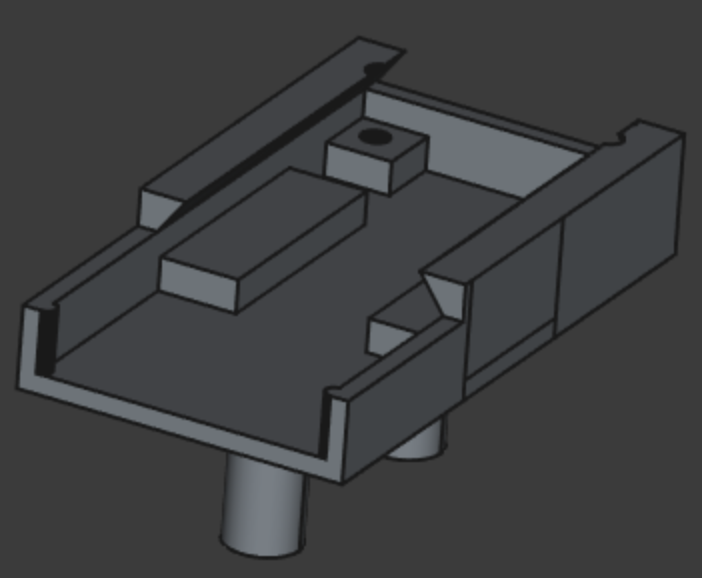
\includegraphics[width=0.35\textwidth, keepaspectratio]{images/becker_cad_flywheel.png}
    \caption{Halterung für Flywheel Motortreiber}
\end{figure}

\section{Mikrocontroller-Case (Becker)}

Die Mikrocontroller-Case bietet Platz für einen ESP-32 auf einem Freenove Breakout Board und für einen Raspberry Pi 5 mit aktivem Luftkühler. 
Beide Controller sind in diesem Fall übereinander angeordnet, da auf der Lochplattform ansonsten nicht genügend Platz zur Verfügung stehen würde, um alle weiteren erforderlichen Komponenten, wie beispielsweise jene für die Stromversorgung, unterzubringen. 
Aufgrund der Verwendung fester Kabel, wie beispielsweise des Kamerakabels für den Raspberry PI, und der allgemeinen Kabellänge müssen beide Controller in unmittelbarer Nähe zur Geschützplattform platziert werden.

Der ESP-32 ist im unteren Teil des Gehäuses untergebracht. Im ersten Entwurf wurde lediglich eine Vorlage \cite{cad_esp_case_blueprint} gedruckt. 
Es stellte sich jedoch heraus, dass es von dem Freenve-Steckbrett mehrere Varianten in unterschiedlichen Größen gibt. 
Die gewählte Vorlage erwies sich als zu klein, um unser konkretes Modell darin zu platzieren. 
Daher wurde auf Basis der Vorlage eine Version mit passenden Dimensionen erstellt. 
Darüber hinaus wurden einige Änderungen vorgenommen. So wurde ein zusätzliches Schraubloch hinzugefügt, um eine externe Antenne anzuschließen und somit die Bluetooth- und WLAN-Abdeckung zu optimieren. 
Im nächsten Schritt wurden im Deckel Kühllöcher in Form des Textes HimmelWacht integriert, um den Mikrocontroller mit zusätzlicher Luft zu versorgen.

\begin{figure}[ht]
    \centering
    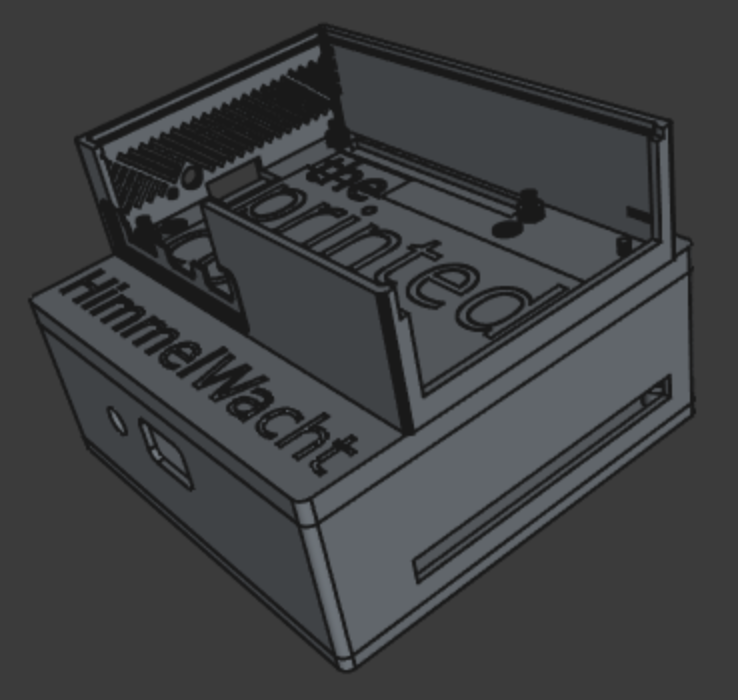
\includegraphics[width=0.45\textwidth, keepaspectratio]{images/becker_cad_esp_case.png}
    \caption{Mikrocontroller Case}
\end{figure}

Zuletzt wurde die Unterseite der Case noch mit dem modularen Stecksystem ausgestattet, welches auch für Teile der Stromversorgung verwendet wird.
Die Montage kann somit ohne den Einsatz von Klebstoff oder Schrauben durchgeführt werden.

\section{Halterung Lautsprecher (Becker)}

Auch für den ursprünglich vorgesehenen Lautsprecher wurde eine Befestigung konstruiert. 
Die vorliegende Halterung wurde konzipiert, um sowohl den Lautsprecher als auch das zugehörige Verstärkerboard unterzubringen, womit kurze Kabellängen und eine damit einhergehend einfachere Verkabelung gewährleistet werden. 
Diese Halterung ist ebenfalls mit dem modularen Stecksystem ausgestattet.


\begin{figure}[ht]
    \centering
    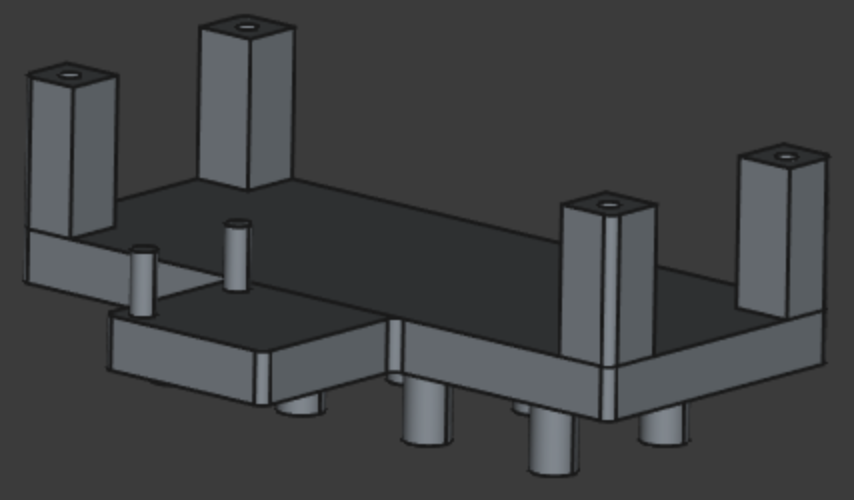
\includegraphics[width=0.45\textwidth, keepaspectratio]{images/becker_cad_speaker.png}
    \caption{Lautsprecherhalterung}
\end{figure}
